
\lecture{Introduction to Probability}{intro-to-probability}
\section{Introduction to Probability}

\title{Probability}
\subtitle{What are the chances?}

%\author{Kelly Black}
%\institute{Clarkson University}
\date{27 August 2014}

\begin{frame}
  \titlepage
\end{frame}

\begin{frame}
  \frametitle{Outline}
  \tableofcontents[hideothersubsections,sectionstyle=show/hide]
\end{frame}


\subsection{Clicker Quiz}


\iftoggle{clicker}{%

  \begin{frame}
    \frametitle{Clicker Quiz}

    If I flip a fair coin ten times how many tails will I get?

    \begin{tabular}{l@{\hspace{3em}}l@{\hspace{3em}}l@{\hspace{3em}}l}
      A: 4 & B: 5 & C: 6 & D: I do not know
    \end{tabular}


  \end{frame}

}




\subsection{Recap From Previous Meeting}

%\begin{frame}
%  \frametitle{Clicker Exercise}
%
%  Flip a coin 3 times. How many tails did you get?
%
%  \begin{tabular}{l@{\hspace{3em}}l@{\hspace{3em}}l@{\hspace{3em}}l}
%  A: 0 & B: 1 & C: 2 & D: 3
%  \end{tabular}
%
%  \only<2->%
%  {
%    Question: What is the probability that we get the same result if
%    we do it again?
%  }
%
%\end{frame}

\begin{frame}{Recall}

  Recall from last time:

  \begin{definition}[Probability]
    ``\textbf{Probability} is the measure of the likelihood of a random
    phenomena or chance behavior. Probability describes the long-term
    proportion with which a certain \textbf{outcome} will occur in
    situations with short-term uncertainty.'' % (Page 223)
  \end{definition}

  
\end{frame}


\begin{frame}{Also Recall}

  \begin{description}
  \item[Event:] Something that \textit{can} happen.
  \item[Outcome:] Something that did happen.
  \item[Experiment:] A structured activity that includes the
    measurement of the outcomes of the activity after predefined and
    intentional changes to some aspect of the events.
  \item[Observational Study:] A structured activity that includes the
    measurement of the outcomes of the activity without intentional
    changes to the events.
  \item[Expected Outcome:] The ``average'' of the possible outcomes.
  \item[Variation:] Some measure of the spread of possible outcomes.
  \end{description}
  
\end{frame}

\begin{frame}{Also Also Recall}

  ``Probability'' is an idealized notion. If we repeat the experiment
  an infinite number of times we ask what \textit{will} happen.

  \vfill

  ``Statistics'' is the study of how to interpret data. We ask what
  ``did'' happen and what does it imply about the underlying
  probabilities?

  \vfill

\end{frame}


\subsection{Events}

\begin{frame}
  \frametitle{Events}

  \begin{definition}
    An event is a possible outcome from an experiment.
  \end{definition}

\end{frame}


\begin{frame}
  \frametitle{Sample Space}

  \begin{definition}
    The sample space is the collection of all possible events.
  \end{definition}

\end{frame}


\begin{frame}
  \frametitle{Sample Space}

  There are two ways to visualize the sample space:
  \begin{itemize}
  \item Venn Diagram
  \item Tree Diagram
  \end{itemize}

\end{frame}

\subsection{Sample Space Examples}

\begin{frame}{Example}

  We flip a coin two times. What are the events?

  \only<2->%
  {

    \begin{eqnarray*}
      p(\mathrm{first~T}) & = & ? \\
      p(TT) & = & ? \\
      p(TH) & = & ? \\
      p(\mathrm{second~H}) & = & ? \\
      p(\mathrm{one~T}) & = & ? \\
      p(\mathrm{two~H}) & = & ?
    \end{eqnarray*}

  }
  
\end{frame}

\begin{frame}{Example}

  We flip a coin two times. What are the events?

  \begin{columns}
    \column{.5\textwidth}

    \begin{picture}(100,100)
      \put(0,0){\line(1,0){100}}
      \put(100,0){\line(0,1){100}}
      \put(0,0){\line(0,1){100}}
      \put(0,100){\line(1,0){100}}
      \put(50,0){\line(0,1){100}}
      \put(0,50){\line(1,0){100}}

      \put(20,20){TT}
      \put(20,70){HT}
      \put(70,70){HH}
      \put(70,20){TH}

    \end{picture}


    \column{.5\textwidth}

    \begin{picture}(100,100)
      \put(0,50){\circle*{2}}

      \put(0,50){\line(1,1){20}}
      \put(22,68){T}
      \put(0,50){\line(1,-1){20}}
      \put(22,25){H}

      \put(35,75){\circle*{2}}
      \put(35,75){\line(2,1){20}}
      \put(59,85){T}
      \put(35,75){\line(2,-1){20}}
      \put(59,60){H}

      \put(35,30){\circle*{2}}
      \put(35,30){\line(2,1){20}}
      \put(59,40){T}
      \put(35,30){\line(2,-1){20}}
      \put(59,15){H}

    \end{picture}



  \end{columns}
  
\end{frame}


\begin{frame}{Clicker Quiz}
  A couple has a child. Two years later they have another child. What
  is the probability that they have one girl and one boy?

  \begin{tabular}{l@{\hspace{3em}}l@{\hspace{3em}}l@{\hspace{3em}}l}
    A: 0 & B: 1/4 & C: 1/2 & D: 1
  \end{tabular}

\end{frame}

\begin{frame}{Example}

  I roll a fair three sided die twice. What is $p(\mathrm{sum}=2)$?
  
\end{frame}

\subsection{The Compliment}

\begin{frame}{The Compliment}

  \begin{columns}
    \column{.5\textwidth}
    \begin{definition}[The Compliment]
      The compliment of an event, $A$, is the set of all events not in
      $A$.  The compliment of a set, $A$, is denoted $A'$. (Other
      notations: $\bar{A}$ or $A^c$ or others.)
    \end{definition}

    \column{.5\textwidth}
    \centerline{\includegraphics[width=4cm]{img/compliment}}
  \end{columns}
\end{frame}

\begin{frame}{Example}
  You meet two unrelated people. What is the probability that their
  birthdays are not on the same day?
\end{frame}


\subsection{Combining Events}

\begin{frame}{The Intersection}

  \begin{columns}
    \column{.5\textwidth}
    \begin{definition}[Intersection]
      The intersection of two events, $A$ and $B$, is the set of all
      events that are in both $A$ \textbf{and} $B$.
    \end{definition}
    \column{.5\textwidth}
    Notation:
    \begin{eqnarray*}
      p(A\cap B) & = & \mathrm{Probability~that~an} \\
                 &   & \mathrm{~event~in~both} \\
                 &   & \mathrm{~A~and~B~occurs.}
    \end{eqnarray*}
  \end{columns}
\end{frame}


\begin{frame}{The Union}

  \begin{columns}
    \column{.5\textwidth}
    \begin{definition}[Union]
      The union of two events, $A$ and $B$, is the set of all
      events that are in either $A$ \textbf{or} $B$.
    \end{definition}
    \column{.5\textwidth}
    Notation:
    \begin{eqnarray*}
      p(A\cup B) & = & \mathrm{Probability~that~an} \\
                 &   & \mathrm{~event~in~either} \\
                 &   & \mathrm{~A~or~B~occurs.}
    \end{eqnarray*}
  \end{columns}
\end{frame}

\begin{frame}{Example}

  \centerline{\includegraphics[width=6cm]{img/vennProbability}}
  
\end{frame}

\begin{frame}{Identities}

  \begin{eqnarray*}
    p(A \cup B) & = & p(A) + p(B) - p(A \cap B), \\
    \uncover<2>{
      p(A \cup B \cup C) & = & p(A) + p(B) + p(C) \\
      & & - p(A \cap B) - p(B \cap C) - p(C \cap A) \\
      & & + p(A \cap B \cap C).
    }
  \end{eqnarray*}
  
\end{frame}


% LocalWords:  Clarkson pausesection hideallsubsections
